\documentclass[12pt]{article}
\usepackage{amsmath}
\usepackage{amssymb}
\usepackage[letterpaper,margin=0.85in,centering]{geometry}
\usepackage{fancyhdr}
\usepackage{enumerate}
\usepackage{lastpage}
\usepackage{multicol}
\usepackage{graphicx}
\usepackage{tikz}
\usetikzlibrary{calc, positioning, decorations.pathmorphing}

\reversemarginpar

\pagestyle{fancy}
\cfoot{}
\lhead{Math 1560}\chead{Tutorial Assignment \# 2}\rhead{May 16th, 2017}
%\rfoot{Total: 10 points}
%\chead{{\bf Name:}}
\newcommand{\points}[1]{\marginpar{\hspace{24pt}[#1]}}
\newcommand{\skipline}{\vspace{12pt}}
%\renewcommand{\headrulewidth}{0in}
\headheight 30pt

\newcommand{\di}{\displaystyle}
\newcommand{\abs}[1]{\lvert #1\rvert}
\newcommand{\len}[1]{\lVert #1\rVert}
\renewcommand{\i}{\mathbf{i}}
\renewcommand{\j}{\mathbf{j}}
\renewcommand{\k}{\mathbf{k}}
\newcommand{\R}{\mathbb{R}}
\newcommand{\aaa}{\mathbf{a}}
\newcommand{\bbb}{\mathbf{b}}
\newcommand{\ccc}{\mathbf{c}}
\newcommand{\dotp}{\boldsymbol{\cdot}}
\newcommand{\bbm}{\begin{bmatrix}}
\newcommand{\ebm}{\end{bmatrix}}                   
                  
\begin{document}
{\bf \large Name:} \hspace{2.5in} {\bf Tutorial time:}

\bigskip

\bigskip

%\author{Instructor: Sean Fitzpatrick}
\thispagestyle{fancy}
%\noindent{{\bf Name and student number:}}

 \begin{enumerate}
 \item  Evaluate the following limits:
\begin{enumerate}
 \item \begin{align*} \lim_{x\to 2}\frac{2-\sqrt{x+2}}{x-2} & = \lim_{x\to 2}\frac{(2-\sqrt{x+2})(2+\sqrt{x+2})}{(x-2)(2+\sqrt{x+2})}\\
        & = \lim_{x\to 2}\frac{2-(x+2)}{(x-2)(2+\sqrt{x+2})}\\
        & = \lim_{x\to 2}\frac{(-1)}{2+\sqrt{x+2}} = \frac{-1}{2+\sqrt{4}} = -\frac{1}{4}.
       \end{align*}


 \item \begin{align*} \lim_{\theta\to 0}\frac{\tan\theta}{\sin\theta + 2\theta} & = \lim_{\theta\to 0}\frac{\frac{1}{\theta}(\tan\theta)}{\frac{1}{\theta}(\sin\theta+2\theta)}\\[4pt]
        & = \lim_{\theta\to 0}\frac{\left(\frac{\sin\theta}{\theta}\right)\frac{1}{\cos\theta}}{\frac{\sin\theta}{\theta}+2}\\[4pt]
	& = \frac{\lim_{\theta\to 0}\left(\frac{\sin\theta}{\theta}\right)\frac{1}{\lim_{\theta\to 0}\cos\theta}}{\lim_{\theta\to 0}\left(\frac{\sin\theta}{\theta}\right)+2}\\[4pt]
	& = \frac{1(1)}{1+2} = \frac{1}{3}.
       \end{align*}


 \item $\di \lim_{x\to 0}x^2\cos\left(\frac{1}{x^2}\right)$ (Hint: squeeze theorem)

\medskip

Since $-1\leq \cos(1/x^2)\leq 1$ for all $x\neq 0$, it follows that
\[
 -x^2\leq x^2\cos(1/x^2)\leq x^2
\]
for all $x\neq 0$. Since $\lim_{x\to 0}(-x^2) = \lim_{x\to 0}(x^2) =0$, it follows from the squeeze theorem that $\di \lim_{x\to 0}x^2\cos(1/x^2)=0$.

\bigskip

 \item $\di \lim_{x\to 2^+}\frac{x^2-9}{x^2-4}$.

\medskip

Since the denominator is zero at $x=2$ but the numerator is not, we must have a vertical asymptote at $x=2$. We note that $\dfrac{x^2-9}{x^2-4} = \dfrac{(x-3)(x+3)}{(x-2)(x+2)}$ is negative for $2<x<3$. (Verify using a sign diagram.) It follows that
\[
 \lim_{x\to 2^+}\frac{x^2-9}{x^2-4} = -\infty.
\]

\end{enumerate}

\newpage

 \item Let $f(x) = \dfrac{x^2-4}{x^2-4x+3}$.
\begin{enumerate}
 \item What is the horizontal asymptote for the graph $y=f(x)$?

\medskip

The highest power of $x$ top and bottom is 2, and both $x^2$ terms have a coefficient of 1, so there is a horizontal asymptote at $y=1$.

\medskip

 \item What are the vertical asymptotes for the graph $y=f(x)$?

\medskip

The denominator $x^2-4x+3 = (x-1)(x-3)$ is equal zero for $x=1$ and $x=3$. Since the numerator is non-zero at both of these values, both $x=1$ and $x=3$ are vertical asymptotes.

\medskip

 \item What are the left and right-hand limits of $f(x)$ at each vertical asymptote?

From the sign diagram
\begin{center}
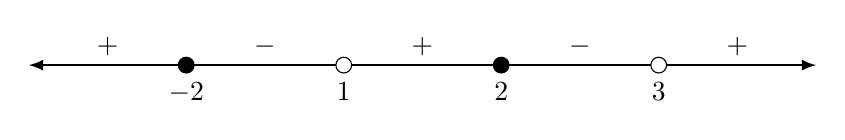
\begin{tikzpicture}[>=latex]
  \draw [thick, <->] (-5,0) -- (5,0);
  \draw [fill] (-3,0) circle [radius =.1];
  \draw [fill=white] (-1,0) circle [radius =.1];
  \draw [fill] (1,0) circle [radius =.1];
  \draw [fill=white] (3,0) circle [radius =.1];
  \node at (-4,0) [above] {$+$};
  \node at (-2,0) [above] {$-$};
  \node at (-0,0) [above] {$+$};
  \node at (2,0) [above] {$-$};
  \node at (4,0) [above] {$+$};
  \node at (-3,-0.1) [below] {$-2$};
  \node at (-1,-0.1) [below] {$1$};
  \node at (1,-0.1) [below] {$2$};
  \node at (3,-0.1) [below] {$3$};
  \end{tikzpicture}
\end{center}
\end{enumerate}
we can read off the desired limits:
\[
 \lim_{x\to 1^-}f(x) = -\infty,\, \lim_{x\to 1^+}f(x) = \infty,\, \lim_{x\to 3^-}f(x) = -\infty,\,\text{ and } \lim_{x\to 3^+}f(x) = \infty.
\]




\item Find and classify the discontinuities of $\di f(x) = \begin{cases} \frac{x^2+2x+1}{x+1}, & \text{ if } x \leq 0\\ \frac{1}{x-2}, & \text{ if } x>0\end{cases}$

\medskip

We note that $\frac{x^2+2x+1}{x+1} = \frac{(x+1)^2}{x+1} = x+1$ for $x\neq -1$. Thus $f(-1)$ is undefined, but the limit at $-1$ exists, so there is a removable discontinuity at $x=-1$. Since $\lim_{x\to 0^-}f(x) = \frac{0^2+2(0)+1}{0+1} = 1$ but $\lim_{x\to 0^+}f(x) = \frac{1}{0-2} = -\frac{1}{2}$, there is a jump discontinuity at $x=0$. Finally, we can easily see that there is a vertical asymptote at $x=2$, so there is an infinite discontinuity at this point.

\medskip

\item Using the \textbf{definition} of the derivative, find the equation of the tangent line to $y=x^2+1$ at the point $(1,2)$.

\medskip

By definition, for $f(x)=x^2+1$ we have:
\[
 f'(1) = \lim_{h\to 0}\frac{((1+h)^2+1)-(1^2+1)}{h} = \lim_{h\to 0}\frac{1+2h+h^2+1-2}{h} = \lim_{x\to 0}(2+h) = 2.
\]
Since $f'(1)$ gives the slope of the tangent line at $x=1$, we have the equation $y-2 = 2(x-1)$, or $y=2x$, for the tangent line.
 \end{enumerate}
\end{document}